\chapter{\inverseMatTitle}
\label{inverse_matrix}


\begin{definition}
A square matrix $M$ is \emph{invertible} (or \emph{nonsingular})\index{Invertible}\index{Nonsingular} if there exists a matrix $M^{-1}$ such that
\[
M^{-1}M=I=M^{-1}M.
\]
\end{definition}

%\begin{figure}
%\begin{center}
%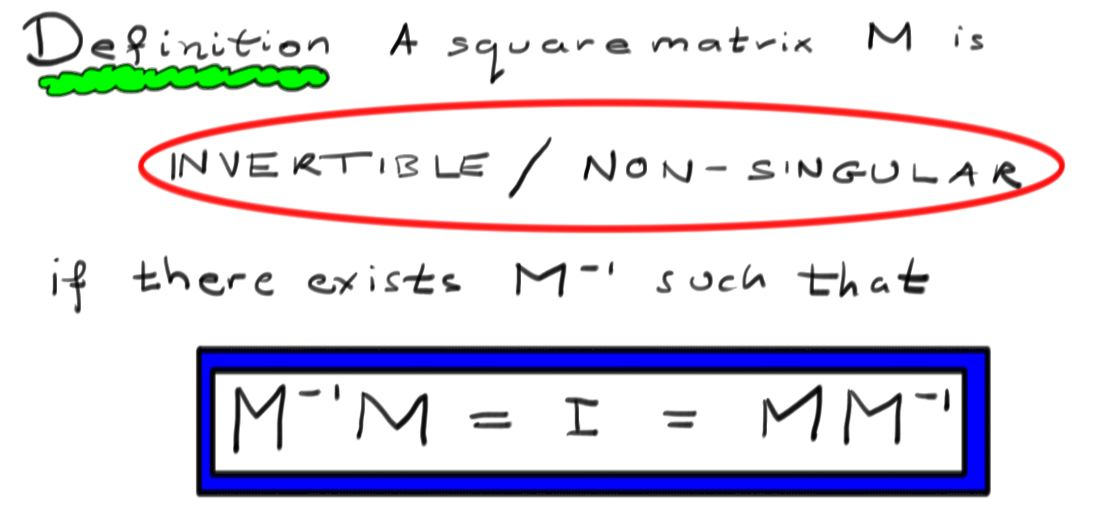
\includegraphics[scale=.27]{\inverseMatPath/defn_inverse_matrix.jpg}
%\end{center}
%\end{figure}


\begin{remark}[Inverse of a $2\times 2$ Matrix] Let $M$ and $N$ be the matrices:
\[
M=\begin{pmatrix}
a & b \\
c & d \\
\end{pmatrix},\qquad N=\begin{pmatrix}
d & -b \\
-c & a \\
\end{pmatrix}
\]
Multiplying these matrices gives:
\[
MN=\begin{pmatrix}
ad-bc & 0 \\
0 & ad-bc \\
\end{pmatrix}=(ad-bc)I
\]

Then $M^{-1}=\frac{1}{ad-bc}\begin{pmatrix}
d & -b \\
-c & a \\
\end{pmatrix}$, so long as $ad-bc\neq 0$.    
\end{remark}

\begin{figure}
\begin{center}
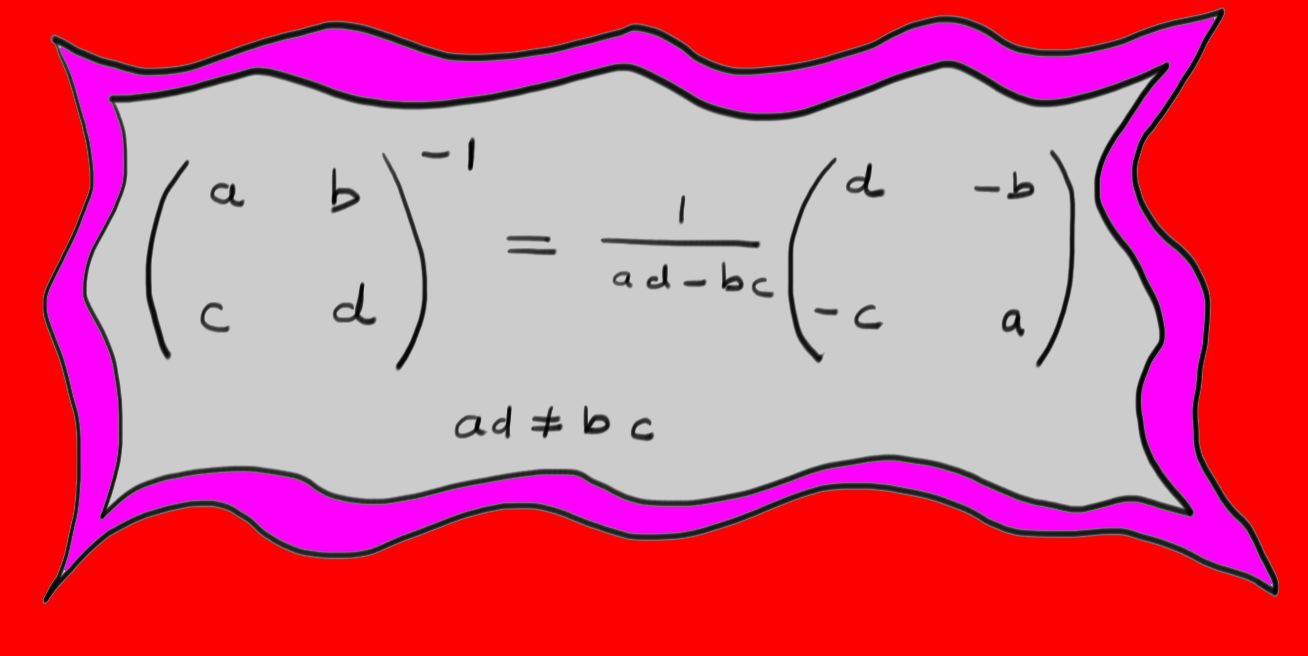
\includegraphics[scale=.24]{\inverseMatPath/2x2_inverse.jpg}
\end{center}
\caption{The formula for the inverse of a 2$\times$2 matrix is worth memorizing!}
\end{figure}



\section{Three Properties of the Inverse}

\begin{enumerate}
\item If $A$ is a square matrix and $B$ is the inverse of $A$, then $A$ is the inverse of $B$, since $AB=I=BA$.  Then we have the identity:
\[
(A^{-1})^{-1}=A
\]

\item Notice that $B^{-1}A^{-1}AB=B^{-1}IB=I=ABB^{-1}A^{-1}$.
Then:
\[
(AB)^{-1}=B^{-1}A^{-1}
\]
Then much like the transpose, taking the inverse of a product \emph{reverses} the order of the product.


\begin{center}
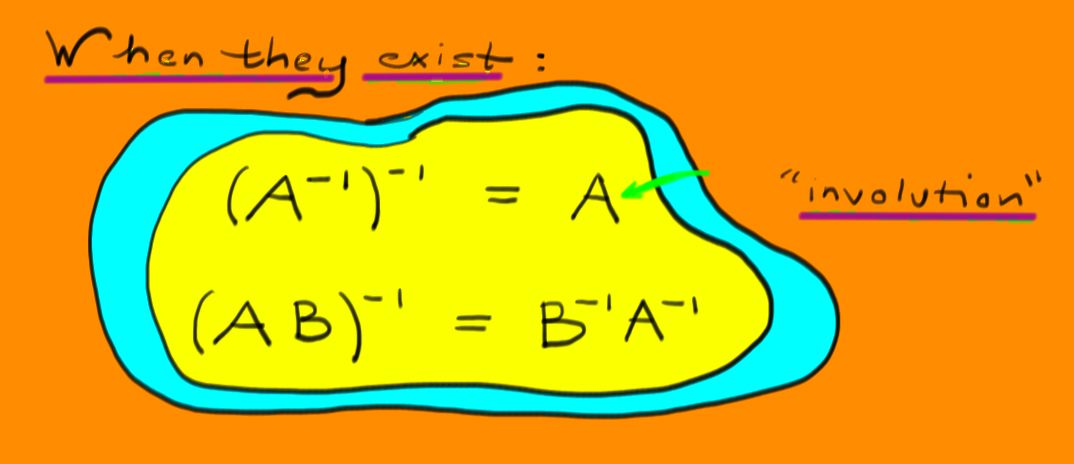
\includegraphics[scale=.26]{\inverseMatPath/inverse_inverse.jpg}
\end{center}

\item Finally, recall that $(AB)^T=B^TA^T$.  Since $I^T=I$, then $(A^{-1}A)^T=A^T(A^{-1})^T=I$.  Similarly, $(AA^{-1})^T=(A^{-1})^TA^T=I$.  Then:
\[
(A^{-1})^T=(A^T)^{-1}
\]
%As such, we could even write $A^{-T}$ for the inverse of the transpose of $A$ (or equivalently the transpose of the inverse).
\begin{center}
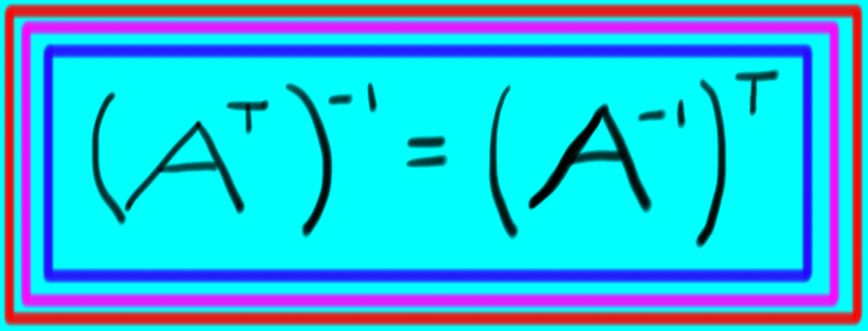
\includegraphics[scale=.20]{\inverseMatPath/transpose_inverse.jpg}
\end{center}
\end{enumerate}

\videoscriptlink{inverse_matrix_2by2_example.mp4}{Example}{scripts_inverse_matrix_2by2_example}




\section{Finding Inverses}

Suppose $M$ is a square matrix and $MX=V$ is a linear system with unique solution $X_0$.  Since there is a unique solution, $M^{-1}V$, then the reduced row echelon form of the linear system has an identity matrix on the left:
\[
\begin{amatrix}{1}
M & V
\end{amatrix}
\sim
\begin{amatrix}{1}
I & M^{-1}V
\end{amatrix}
\]
Solving the linear system $MX=V$ then tells us what $M^{-1}V$ is.  

To solve many linear systems with the same matrix at once, 
$$MX=V_1,~MX=V_2$$

we can consider augmented matrices with 
%a matrix on the right side instead of a column vector, 
many columns on the right 
 and then apply Gaussian row reduction to the left side of the matrix.  Once the identity matrix is on the left side of the augmented matrix, then the solution of each of the individual linear systems is on the right.
 \[
\left(\begin{array}{c|cc}
M & V_1&V_2
\end{array}\right)
\sim
\left(\begin{array}{c|cc}
I & M^{-1}V_1 & M^{-1}V_2
\end{array}\right)
\]


To compute $M^{-1}$, we would like $M^{-1}$, rather than $M^{-1}V$ to appear on the right side of our augmented matrix.
This is achieved by  solving the collection of systems $MX=e_k$, where $e_k$ is the column vector of zeroes with a $1$ in the $k$th entry.  
{\it I.e.,} the $n\times n$ identity matrix can be viewed as a bunch of column vectors $I_n=(e_1 \ e_2 \ \cdots e_n)$. So, putting the $e_k$'s together into an identity matrix, we get:
\[
\begin{amatrix}{1}
M & I
\end{amatrix}
\sim
\begin{amatrix}{1}
I & M^{-1}I
\end{amatrix}
=\begin{amatrix}{1}
I & M^{-1}
\end{amatrix}
\]


\begin{example}
Find $\begin{pmatrix}
-1 & 2 & -3 \\
2 & 1 & 0 \\
4 & -2 & 5 \\
\end{pmatrix}^{-1}
$.
Start by writing the augmented matrix, then apply row reduction to the left side.

\begin{eqnarray*}
\begin{pmat}{rrr|ccc}
-1 & 2 & -3 & 1 & 0 & 0 \\[1mm]
2  & 1 &  0 & 0 & 1 & 0 \\[1mm]
 4 & -2 & 5 & 0 & 0 & 1 \\[1mm]
\end{pmat} & \sim & \begin{pmat}{crr|ccc}
1  & -2&  3  & 1 & 0 & 0 \\[1mm]
0  & 5 &  -6 & 2 & 1 & 0 \\[1mm]
 0 & 6 & -7  & 4 & 0 & 1 \\[1mm]
\end{pmat} \\[2mm]
& \sim & \begin{pmat}{ccr|rrc}
1  & 0 &  \frac{3}{5}  & -\frac{1}{4} & \frac{2}{5} & 0 \\[1mm]
0  & 1 &  -\frac{6}{5} & \frac{2}{5} & \frac{1}{5}  & 0 \\[1mm]
 0 & 0 &  \frac{1}{5}  & \frac{4}{5} & -\frac{6}{5} & 1 \\[1mm]
\end{pmat} \\[2mm]
& \sim & \begin{pmat}{ccc|rrr}
1  & 0 &  0  & -5 & 4 & -3 \\[1mm]
0  & 1 &  0  & 10 & -7 & 6 \\[1mm]
 0 & 0 &  1  & 8 & -6 & 5 \\[1mm]
\end{pmat} \\
\end{eqnarray*}
At this point, we know $M^{-1}$ assuming we didn't goof up\index{Goofing up}.  However, row reduction is a lengthy and arithmetically involved process, so we should~\emph{check our answer,} by confirming that $MM^{-1}=I$ (or if you prefer $M^{-1}M=I$):
\[MM^{-1} = 
\begin{pmatrix}
-1 & 2 & -3 \\
2 & 1 & 0 \\
4 & -2 & 5 \\
\end{pmatrix}\begin{pmatrix}
-5 & 4 & -3 \\
10 & -7 & 6 \\
 8 & -6 & 5 \\
\end{pmatrix}
=\begin{pmatrix}
1 & 0 & 0 \\
0 & 1 & 0 \\
0 & 0 & 1 \\
\end{pmatrix}
\]  
The product of the two matrices is indeed the identity matrix, so we're done.
\end{example}

%\href{\webworkurl ReadingHomework10/1/}{Reading homework: problem 10.1}
\reading{10}{1}
\section{Linear Systems and Inverses}

If $M^{-1}$ exists and is known, then we can immediately solve linear systems associated to $M$.

\begin{example}
Consider the linear system:

\[
      \begin{linsys}{2}
            -x & +2y & -3z         &=& 1  \\[1mm]
            2x & +\ y\,   &             &=& 2 \\[1mm]
            4x & -2y & +5z         &=& 0  
      \end{linsys}
\]
The associated matrix equation is $MX=\colvec{1\\2\\0},$ where \(M\) is the same as in the previous section.  Then:

\[
\colvec{x\\y\\z}=\begin{pmatrix}
-1 & 2 & -3 \\
2 & 1 & 0 \\
4 & -2 & 5 \\
\end{pmatrix}^{-1}\colvec{1\\2\\0}
=\begin{pmatrix}
-5 & 4 & -3 \\
10 & -7 & 6 \\
 8 & -6 & 5 \\
\end{pmatrix}\colvec{1\\2\\0}
=\colvec{3\\-4\\-4}
\]
Then $\colvec{x\\y\\z}=\colvec{3\\-4\\-4}$.  
In summary, when $M^{-1}$ exists, then $$MX=V \Rightarrow X=M^{-1}V\, .$$
\end{example}



%\href{\webworkurl ReadingHomework10/2/}{Reading homework: problem 10.2}
\reading{10}{2}

\section{Homogeneous Systems}

\begin{theorem}
A square matrix $M$ is invertible if and only if the homogeneous system $$MX=0$$ has no non-zero solutions.
\end{theorem}

\begin{proof}
First, suppose that $M^{-1}$ exists.  Then $MX=0 \Rightarrow X=M^{-1}0=0$.  Thus, if $M$ is invertible, then $MX=0$ has no non-zero solutions.

On the other hand, $MX=0$ always has the solution $X=0$.  If no other solutions exist, then $M$ can be put into reduced row echelon form with every variable a pivot.  In this case, $M^{-1}$ can be computed using the process in the previous section.
\end{proof}

%\begin{figure}
\begin{center}
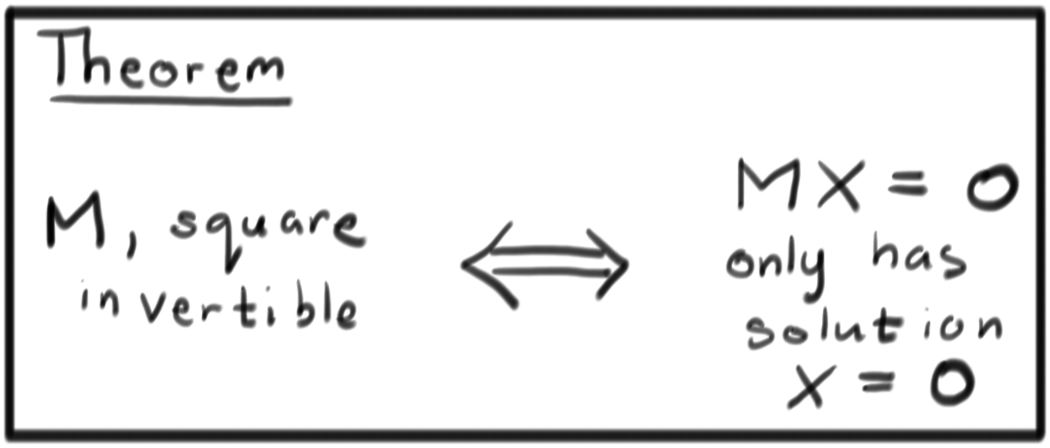
\includegraphics[scale=.26]{\inverseMatPath/inverse_theorem.jpg}
\end{center}
%\end{figure}

%A great test of your linear algebra knowledge is to make a list of conditions for a matrix to be singular.
%You will learn more of these as the course goes by, but can also skip straight to the list in Section~\ref{thelist}. 

\section{Bit Matrices}\index{Bit matrices}
In computer science, information is recorded using binary strings of data.  For example, the following string contains an English word:
\[
011011000110100101101110011001010110000101110010
\]
A \hypertarget{bits}{\emph{bit}} is the basic unit of information, keeping track of a single one or zero.  Computers can add and multiply individual bits very quickly.

Consider the set $\Z_2=\{0,1 \}$ with addition and multiplication given by the following tables:
\label{Z2}
\[
\begin{array}{c|cc}
+ & 0 & 1 \\ \hline
0 & 0 & 1 \\
1 & 1 & 0 \\
\end{array}
\qquad
\begin{array}{c|cc}
\cdot & 0 & 1 \\ \hline
0 & 0 & 0 \\
1 & 0 & 1 \\
\end{array}
\]
Notice that $-1=1$, since $1+1=0$.

It turns out that $\Z_2$ is almost as good as the real or complex numbers (they are all \hyperref[fields]{fields}), so we can apply all of the linear algebra we have learned thus far to matrices with $\Z_2$ entries.  A matrix with entries in $\Z_2$ is sometimes called a \emph{bit matrix}\footnote{Note that bits in a bit arithmetic shorthand do not ``add'' and ``multiply'' as elements in $\mathbb{Z}_2$ does since these operators corresponding to ``bitwise or'' and ``bitwise and'' respectively.}.

\begin{example}
$\begin{pmatrix}
1 & 0 & 1 \\
0 & 1 & 1 \\
1 & 1 & 1 \\
\end{pmatrix}$ is an invertible matrix over $\Z_2$:

\[\begin{pmatrix}
1 & 0 & 1 \\
0 & 1 & 1 \\
1 & 1 & 1 \\
\end{pmatrix}^{-1}=\begin{pmatrix}
0 & 1 & 1 \\
1 & 0 & 1 \\
1 & 1 & 1 \\
\end{pmatrix}
\]

This can be easily verified by multiplying:

\[\begin{pmatrix}
1 & 0 & 1 \\
0 & 1 & 1 \\
1 & 1 & 1 \\
\end{pmatrix}\begin{pmatrix}
0 & 1 & 1 \\
1 & 0 & 1 \\
1 & 1 & 1 \\
\end{pmatrix}=\begin{pmatrix}
1 & 0 & 0 \\
0 & 1 & 0 \\
0 & 0 & 1 \\
\end{pmatrix}
\]
\end{example}

\begin{remark}[Application: Cryptography]  
A very simple way to hide information is to use a substitution cipher, in which the alphabet is permuted and each letter in a message is systematically exchanged for another.  For example, the ROT-13 cypher just exchanges a letter with the letter thirteen places before or after it in the alphabet.  For example, HELLO becomes URYYB.  Applying the algorithm again decodes the message, turning URYYB back into HELLO.  Substitution ciphers are easy to break, but the basic idea can be extended to create cryptographic systems that are practically uncrackable.  For example, a \emph{one-time pad} is a system that uses a different substitution for each letter in the message.  So long as a particular set of substitutions is not used on more than one message, the one-time pad is unbreakable.

English characters are often stored in computers in the ASCII format.  In ASCII, a single character is represented by a string of eight bits, which we can consider as a vector in $\Z_2^8$ (which is like vectors in $\Re^8$, where the entries are zeros and ones).  One way to create a substitution cipher, then, is to choose an $8\times 8$ invertible bit matrix $M$, and multiply each letter of the message by $M$.  Then to decode the message, each string of eight characters would be multiplied by $M^{-1}$.  

To make the message a bit tougher to decode, one could consider pairs (or longer sequences) of letters as a single vector in $\Z_2^{16}$ (or a higher-dimensional space), and then use an appropriately-sized invertible matrix.

For more on cryptography, see ``The Code Book,'' by Simon Singh (1999, Doubleday).
\end{remark}

%{\it You should now be ready to attempt the \hyperref[sample1]{first sample midterm}.}
%\begin{center}
%\shabox{
%\begin{tabular}{c}
%\it \hyperref[sample1]{You are now ready to attempt the first sample midterm}. 
%\\
%\hyperref[sample1]{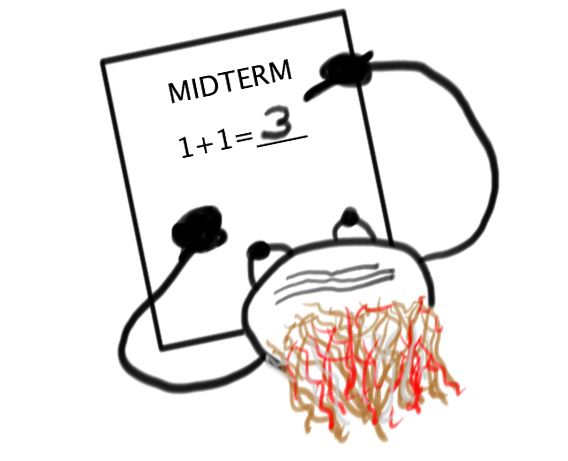
\includegraphics[scale=.15]{midterm.jpg}}
%\end{tabular}
%}
%\end{center}
%
%\section*{References}
%
%Hefferon: Chapter Three, Section IV.2
%\\
%Beezer: Chapter M, Section MISLE
%\\
%Wikipedia:
%\href{http://en.wikipedia.org/wiki/Invertible_matrix}{Invertible Matrix}
%
%
\section{Review Problems}



\begin{enumerate}

\item Let $D=\begin{pmatrix}
\lambda_1 & \mc0 \\
\mc0 & \lambda_2 \\
\end{pmatrix}$.
\begin{enumerate}
\item Write $D$ in terms of the vectors $e_1$ and $e_2$, and their transposes.
\item Suppose $P=\begin{pmatrix}
a & b \\
c & d \\
\end{pmatrix}$ is invertible.  Show that $D$ is similar to
\[
M=\frac{1}{ad-bc}\begin{pmatrix}
\lambda_1ad-\lambda_2bc & -(\lambda_1-\lambda_2)ab \\[1mm]
(\lambda_1-\lambda_2)cd & -\lambda_1bc + \lambda_2ad
\end{pmatrix}.
\]
\item Suppose the vectors $\rowvec{a,b}$ and $\rowvec{c,d}$ are orthogonal.  What can you say about $M$ in this case? (Hint: think about what \(M^T\) is equal to.)
\end{enumerate}

\phantomnewpage

\item \label{orthogprob} Suppose $S=\{v_1, \ldots, v_n \}$ is an \emph{orthogonal} (not orthonormal) basis for~$\Re^n$.  Then we can write any vector $v$ as $v=\sum_ic^iv_i$ for some constants $c^i$.  Find a formula for the constants $c^i$ in terms of $v$ and the vectors in~$S$.

\Videoscriptlink{orthonormal_bases_hint.mp4}{Hint}{scripts_orthonormal_bases_hint}
\phantomnewpage

\item \label{orthogprojprob} Let $u,v$ be linearly independent vectors in $\Re^3$, and $P=\spa \{ u,v\}$ be the plane spanned by $u$ and $v$.  
\begin{enumerate}
\item Is the vector $v^\bot := v-\frac{u\cdot v}{u\cdot u}u$ in the plane $P$?
\item  What is the (cosine of the) angle between $v^\bot$ and $u$?
\item %Given your solution to the above, 
How can you find a third vector perpendicular to both $u$ and $v^\bot$?
\item  Construct an orthonormal basis for $\Re^3$ from $u$ and $v$.
\item  Test your abstract formul\ae\ starting with 
\[
u=\rowvec{1 , 2 , 0} \text{ and } v=\rowvec{0 , 1 , 1}.
\]
\end{enumerate}

\Videoscriptlink{orthonormal_bases_hint3.mp4}{Hint}{scripts_orthonormal_bases_hint3}

\phantomnewpage



\item Find an orthonormal  basis for $\Re^4$ which includes $(1,1,1,1)$ using the following procedure:\\
\begin{enumerate} 
\item Pick a vector perpendicular to the vector 
$$v_1 =\colvec{1\\1\\1\\1}$$ from the solution set of the matrix equation $$v_1^Tx=0\, .$$ Pick the vector $v_2$ obtained from the standard Gaussian elimination procedure which is the coefficient of $x_2$.
\item Pick a vector perpendicular to both $v_1$ and $v_2$ from the solutions set of the matrix equation $$\colvec{v_1^T\\[1mm]v_2^T}x=0\, .$$ Pick the vector $v_3$ obtained from the standard Gaussian elimination procedure with $x_3$ as the coefficient. 
\item Pick a vector perpendicular to $v_1,v_2,$ and $v_3$ from the solution set of the matrix equation $$\colvec{v_1^T\\[1mm]v_2^T\\[1mm]v_3^T}x=0\, .$$  Pick the vector $v_4$ obtained from the standard Gaussian elimination procedure with $x_3$ as the coefficient. 
\item Normalize the four vectors obtained   above.
\end{enumerate}


\item Use the inner product $$f\cdot g := \int_0^1 f(x)g(x)dx$$  on the vector space $V={\rm span} \{1,x,x^2,x^3\}$ to perform the Gram-Schmidt procedure on the set of vectors $\{1,x,x^2,x^3\}$. 

\item Use the inner product $$f\cdot g := \int_0^{2\pi} f(x)g(x)dx$$  on the vector space $V={\rm span} \{\sin(x),\sin(2x),\sin(3x) \}$ to perform the Gram-Schmidt procedure on the set of vectors $\{\sin(x),\sin(2x),\sin(3x) \}$. \\
Try to build an orthonormal basis for the vector space $$\spa \{ \sin(nx)~| ~n\in \N \}\, .$$
%What do you suspect about the vector space $\spa \{ \sin(nx)~| ~n\in \N \}$?\\
%What do you suspect about the vector space $\spa \{ \sin(ax)~|~ a \in \Re \}$?
\item 
\begin{enumerate}
\item
Show that if $Q$ is an orthogonal $n\times n$ matrix, then $$u\dotprod v = (Qu)\dotprod (Qv)\, ,$$ for any $u,v\in \Re^n$. That is, $Q$ preserves the inner product. 
\item Does $Q$ preserve the outer product? 
\item  If the set of vectors $\{ u_1,\dots,u_n\}$ is orthonormal and $\{ \lambda_1,\cdots,\lambda_n\}$ is a set of numbers, 
then what are the eigenvalues and eigenvectors of the matrix
$M=\sum_{i=1}^n \lambda_i u_i u_i^T$? 
\item How would the eigenvectors and eigenvalues of this matrix change if we replaced  $\{ u_1,\dots,u_n\}$ by $\{ Qu_1,\dots,Q u_n\}$?
\end{enumerate}


\item Carefully write out the Gram-Schmidt procedure for the set of vectors 
$$\left\{ \colvec{1\\1\\1}, \colvec{1\\-1\\1}, \colvec{1\\1\\-1} \right\} \, .$$ Is it possible to rescale the second vector obtained in the procedure to a vector with integer components? 


\item 
\label{basisortho}
\begin{enumerate}
\item Suppose $u$ and $v$ are linearly independent.  Show that $u$ and $v^\perp$ are also linearly independent.  Explain why $\{u, v^\perp\}$ is a basis for $\spa \{u,v\}$.



\Videoscriptlink{gram_schmidt_and_orthogonal_complements_hint.mp4}{Hint}{gram_schmidt_and_orthogonal_complements_hint}

\item Repeat the previous problem, but with three independent vectors $u,v,w$
 where $v^\perp$ and $w^\perp$ are as defined by the Gram-Schmidt procedure. 
\end{enumerate}

\phantomnewpage


\item \label{QRprob} Find the $QR$ factorization of
$$
M=\begin{pmatrix}1&0&\phantom{\!-}2\\-1&2&0\\-1&-2&2
\end{pmatrix}\, .
$$

\phantomnewpage

\item Given any three vectors $u,v,w$, when do $v^\perp$ or $w^\perp$ of the Gram--Schmidt procedure vanish?

\phantomnewpage

\item For $U$ a subspace of $W$, use the subspace theorem to check that $U^\perp$ is a subspace of $W$.

\phantomnewpage


\phantomnewpage

\item %(Extra Credit) 
Let $S_n$ and $A_n$ define the space of $n \times n$ symmetric and anti-symmetric matrices, respectively. These are subspaces of the vector space $M^n_n$ of all $n\times n$ matrices. What is $\dim M^n_n$, $\dim S_n$, and $\dim A_n$? Show that $M^n_n = S_n + A_n$. Define an inner product on square matrices
$$
M\cdot N ={\rm tr} MN\, .
$$
Is $A_n^{\perp}=S_n$? Is $M^n_n = S_n \oplus A_n$?

%\emph{Hint: Note that $\dim S_n = \dim U_n$ where $U_n$ is the vector space of all $n \times n$ upper triangular matrices, and also note that $\dim A_n = \dim \widetilde{U}_n$ where $\widetilde{U}_n$ is the vector space of all strictly $n \times n$ upper triangular matrices (\emph{i.e.} the diagonal entries are all 0).}

\item The vector space $V={\rm span} \{ \sin(t),\sin(2t), \sin(3t) , \sin(3t)\}$ has an inner product: 
$$f\cdot g:=\int _0^{2\pi}f(t)g(t) dt\, .$$ Find the orthogonal compliment to $U={\rm span} \{ \sin(t)+\sin(2t) \}$ in $V$. Express $\sin(t)-\sin(2t)$ as  the sum of vectors from $U$ and $U^\perp$.

\end{enumerate}

\phantomnewpage

\newpage


